\newpage
\section{Suggested solutions: Signals and Systems}
\begin{enumerate}
\item

\begin{enumerate}[a)]
\item To check linearity of a system, we check Equation \ref{def:linear_sys}:
\begin{align*}
    \mathcal{T}\{c_{1}V_{1}(t)+c_{2}V_{2}(t)\}&=R^{-1}[c_{1}V_{1}(t)+c_{2}V_{2}(t)], \\
    c_{1}\mathcal{T}\{V_{1}(t)\}+c_{2}\mathcal{T}\{V_{2}(t)\} &=c_{1}R^{-1}[V_{1}(t)]^{2} + c_{2}R^{-1}[V_{2}(t)]^{2},
\end{align*}
these are not equal, so the system is not a linear system. 

\item To check time-invariance for this system, verify Equation \ref{def:timeinv}:
\begin{align*}
    \mathcal{T}\{\mathcal{D}(V(t))\}&=\mathcal{T}\{V(t-\tau)\}=R^{-1}[V(t-\tau)]^{2}, \\
    \mathcal{D}\{\mathcal{T}\{V(t)\}\}&=\mathcal{D}\{R^{-1}[V(t)]^{2}\}=R^{-1}[V(t-\tau)]^{2}.
\end{align*}
Here we get that the outputs are equal, hence the system is time-invariant. 
\end{enumerate}

\item
Consider the discrete-time system defined as:
$$y[n]=\frac{1}{5}\sum_{k=0}^{4}x[n-k].$$

\item[a)]
This system averages $x[n]$ with four of its past values. 

\item[b)] Have that:
\begin{align*}
    \mathcal{T}\{c_{1}x_{1}[n]+c_{2}x_{2}[n]\} &= \frac{1}{5}\sum_{m=0}^{4}[c_{1}x_{1}[n-m]+c_{2}x_{2}[n-m]], \\
    c_{1}\mathcal{T}\{x_{1}[n]\}+c_{2}\mathcal{T}\{x_{2}[n]\}&=c_{1}\frac{1}{5}\sum_{j=0}^{4}x_{1}[n-j]+c_{2}\frac{1}{5}\sum_{k=0}^{4}x_{2}[n-k]
    =\frac{1}{5}\sum_{m=0}^{4}[c_{1}x_{1}[n-m]+c_{2}x_{2}[n-m]].
\end{align*}
In the last, step the two sums were combined into one and the index was renamed to $m$. 
From this we can see that the output are equal, so the system is linear. 

\item[c)] To check time-invariance we calculate:
\begin{align*}
    \mathcal{T}\{\mathcal{D}\{x[n]\}\}&=\mathcal{T}\{x[n-\tau]\}=\frac{1}{5}\sum_{k=0}^{4}x[(n-\tau)-k], \\
    \mathcal{D}\{\mathcal{T}\{x[n]\}\}&=\mathcal{D}\left\{\frac{1}{5}\sum_{k=0}^{4}x[n-k]\right\}=\frac{1}{5}\sum_{k=0}^{4}x[(n-k)-\tau].
\end{align*}
These are equal upon rearranging the parenthesis, hence $\mathcal{T}\{\cdot\}$ is time-invariant. 

\item Consider a time-scaling system of the form $y(t)=x(\alpha t)$, where $x(t)$ is the input signal to the system. 

\begin{enumerate}[a)]
\item If $0<\alpha<1$, the output signal gets stretched, becoming wider. In effect, it reduces the frequency of the original signal. 
To see this compare $\sin(t)$ with $\sin(0.5t)$ as an example. 

\item If $\alpha>1$, the original frequencies are increased by a factor of $\alpha$, giving more oscillations in the signal. 
Again, compare $\sin(t)$ with $\sin(2t)$ as an example.

\item Let's check if the system is linear. Have that:
\begin{align*}
    \mathcal{T}\{c_{1}x_{1}(t)+c_{2}x_{2}(t)\}&= c_{1}x_{1}(\alpha t) + c_{2}x_{2}(\alpha t), \\
    c_{1}\mathcal{T}\{x_{1}(t)\}+c_{2}\mathcal{T}\{x_{2}(t)\}&=c_{1}x_{1}(\alpha t)+c_{2}x_{2}(\alpha t),
\end{align*}
so the system is linear as these are equal.

\item Checking time-invariance:
\begin{align*}
    \mathcal{T}\{\mathcal{D}\{x(t)\}\}&=\mathcal{T}\{x(t-\tau)\}=x(\alpha(t-\tau)), \\
    \mathcal{D}\{\mathcal{T}\{x(t)\}\}&=\mathcal{D}\{x(\alpha t)\}=x(\alpha t-\tau).
\end{align*}
The system is not time-invariant as these do not satisfy Equation \ref{def:timeinv}.
\end{enumerate}

\item Consider the derivative as a system $\mathcal{T}\{x(t)\}=\frac{d}{dt}x(t)$. 
This system is time-invariant and linear. It is linear since:
\begin{align*}
    \mathcal{T}\{c_{1}x_{1}(t)+c_{2}x_{2}(t)\}&=c_{1}\frac{d}{dt}x_{1}(t) + c_{2}\frac{d}{dt}x_{2}(t), \\
    c_{1}\mathcal{T}\{x_{1}(t)\}+c_{2}\mathcal{T}\{x_{2}(t)\}&=c_{1}\frac{d}{dt}x_{1}(t) + c_{2}\frac{d}{dt}x_{2}(t),
\end{align*}
are equal, which follows from the linearity of the differential operator.

For time-invariance, we check the condition in Equation \ref{def:timeinv}:
\begin{align*}
    \mathcal{T}\{\mathcal{D}\{x(t)\}\}&=\mathcal{T}\{x(t-\tau)\}=\frac{d}{dt}x(t-\tau), \\
    \mathcal{D}\{\mathcal{T}\{x(t)\}\}&=\mathcal{D}\left\{\frac{d}{dt}x(t)\right\}=\frac{d}{dt}x(t-\tau).
\end{align*}
Showing that Equation \ref{def:timeinv} holds, hence the system is time-invariant. 

\item The guitar amplifier is a system of the form:
$$y(t)=\begin{cases}
    -\beta, \quad \hspace{0.4cm} \alpha x(t)<-\beta,  \\
    \alpha x(t), \quad |\alpha x(t)|\le \beta, \\
    \beta, \quad \hspace{0.7cm}\alpha x(t)>\beta.
\end{cases}$$
The system is not linear. To show this, find a counter example. The linearity should hold for all signals $x(t)$. 
In particular, consider two signals for which $\alpha x_{1}(t)=\beta$ and $\alpha x_{2}(t)=\beta$. 
For these signals we get:
$$\mathcal{T}\{\alpha x_{1}(t)\}+\mathcal{T}\{\alpha x_{2}(t)\}=\beta+\beta=2\beta,$$
while:
$$\mathcal{T}\{\alpha x_{1}(t)+\alpha x_{2}(t)\}=\mathcal{T}\{\beta+\beta\}=\mathcal{T}\{2\beta\}=\beta,$$
as $2\beta > \beta$ by the last condition, hence we get $\mathcal{T}\{2\beta\}=\beta$. 
Thus, we get a contradiction in that $2\beta=\beta$ for all $\beta$, hence the system is non-linear. 

\item For the guitar amplifier of the form:
\begin{equation*}
y_d(t) = \left\{
  \begin{array}{rcr}
    -\beta & \mathrm{when} & \alpha x(t)<-\beta, \\
    \alpha x(t) & \mathrm{when} & |\alpha x(t)| \le \beta, \\
    \beta & \mathrm{when} & \alpha x(t)>\beta.
\end{array}
\right.
\end{equation*}
Have that:
\begin{align*}
    \mathcal{T}\{\mathcal{D}\{x(t)\}\}&=\mathcal{T}\{x(t-\tau)\}=\begin{cases}
        -\beta, \quad \text{for}\ \alpha x(t-\tau)<-\beta,\\
        \alpha x(t-\tau), \quad \text{for}\ |\alpha x(t-\tau)|\le \beta,\\
        \beta, \quad \text{for}\ \alpha x(t-\tau)>\beta.
    \end{cases} \\
    \mathcal{D}\{\mathcal{T}\{x(t)\}\}&=\mathcal{D}\left\{\begin{cases}
        -\beta, \quad \text{for}\ \alpha x(t)<-\beta,\\
        \alpha x(t), \quad \text{for}\ |\alpha x(t)|\le \beta,\\
        \beta, \quad \text{for}\ \alpha x(t)>\beta.
    \end{cases}\right\}=\begin{cases}
        -\beta, \quad \text{for}\ \alpha x(t-\tau)<-\beta,\\
        \alpha x(t-\tau), \quad \text{for}\ |\alpha x(t-\tau)|\le \beta,\\
        \beta, \quad \text{for}\ \alpha x(t-\tau)>\beta,
    \end{cases} \\ 
\end{align*}
so the system is time-invariant. 

\item Running Listing \ref{lst:audio} and looking at the resulting plot, one can see that the signal has been amplified. 
\lstinputlisting[language=Python,caption={Solution for Exercise 4.7},label=ex4.7,linerange={0-44}]{ch04/code/ex4.7.py}
The output from this system is shown below. 
\begin{figure}
\centering
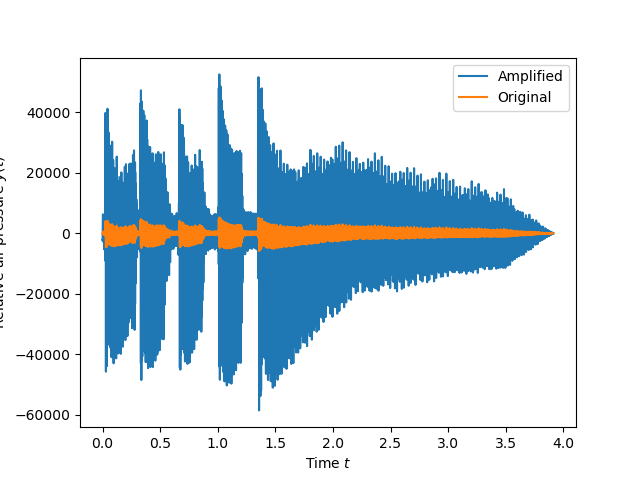
\includegraphics[scale=0.9]{ch04/figures/ex7_plot.png}
\end{figure}

\item Running Listing \ref{ex4.8} applies a distortion effect to the signal. 
\lstinputlisting[language=Python,caption={Solution for Exercise 4.8},label=ex4.8,linerange={0-47}]{ch04/code/ex4.8.py}

\end{enumerate}
